% $Header$
% MBDyn (C) is a multibody analysis code.
% http://www.mbdyn.org
%
% Copyright (C) 1996-2023
%
% Pierangelo Masarati  <pierangelo.masarati@polimi.it>
%
% Dipartimento di Ingegneria Aerospaziale - Politecnico di Milano
% via La Masa, 34 - 20156 Milano, Italy
% http://www.aero.polimi.it
%
% Changing this copyright notice is forbidden.
%
% This program is free software; you can redistribute it and/or modify
% it under the terms of the GNU General Public License as published by
% the Free Software Foundation (version 2 of the License).
% 
%
% This program is distributed in the hope that it will be useful,
% but WITHOUT ANY WARRANTY; without even the implied warranty of
% MERCHANTABILITY or FITNESS FOR A PARTICULAR PURPOSE.  See the
% GNU General Public License for more details.
%
% You should have received a copy of the GNU General Public License
% along with this program; if not, write to the Free Software
% Foundation, Inc., 59 Temple Place, Suite 330, Boston, MA  02111-1307  USA

\section{Beam Elements}
\label{sec:EL:BEAM}
The family of finite volume beam elements implemented in MBDyn
allows to model slender deformable structural components 
with a high level of flexibility.

The beam is defined by a reference line and by a manifold
of orientations attached to the line.
It is assumed that the direction 1 of the orientations lies along
the reference line, but it is not strictly required to be tangent
to it even in the reference configuration.

The beam element is defined by its nodes; currently, 2 and 3 node 
beam elements are implemented.
Each node of the beam is related to a \kw{structural node} by an offset
and an optional relative orientation, to provide topological flexibility.

The beam element is modeled by means of an original Finite Volume approach
\cite{FV-AIAA}, which computes the internal forces as functions 
of the straining of the reference line and orientation at selected points
along the line itself, called \emph{evaluation points},
which lie somewhere between two pairs of beam nodes.

At each evaluation point, a 6D constitutive law must be defined,
which defines the relationship between the strains, the curvatures
of the beam and their time derivatives
and the internal forces and moments at the evaluation points.

The strains and curvatures and their time derivatives are obtained 
from the nodal positions and orientations by differentiating
the interpolation functions.

The 6D constitutive laws are defined as
\begin{displaymath}
	\cubr{\cvvect{
		F_x \\
		F_y \\
		F_z \\
		M_x \\
		M_y \\
		M_z
	}} = \T{f}\plbr{
		\cubr{\cvvect{
			\varepsilon_x \\
			\gamma_y \\
			\gamma_z \\
			\kappa_x \\
			\kappa_y \\
			\kappa_z
		}},
		\cubr{\cvvect{
			\dot{\varepsilon}_x \\
			\dot{\gamma}_y \\
			\dot{\gamma}_z \\
			\dot{\kappa}_x \\
			\dot{\kappa}_y \\
			\dot{\kappa}_z
		}}
	}
\end{displaymath}
where, if the convention of using $x$ as beam axis is followed:
\begin{itemize}
\item $F_x$ is the axial force component;
\item $F_y$ and $F_z$ are the shear force components;
\item $M_x$ is the torsional moment component;
\item $M_y$ and $M_z$ are the bending moment components;
\item $\varepsilon_x$ is the axial strain component;
\item $\gamma_y$ and $\gamma_z$ are the shear strain components;
\item $\kappa_x$ is the torsional curvature component;
\item $\kappa_y$ and $\kappa_z$ are the bending curvature component;
\item $\T{f}$ is an arbitrary function that defines the constitutive law.
\end{itemize}



\subsection{Beam Section Constitutive Law}
Typically, linear elastic or viscoelastic constitutive laws are used,
although one may want to implement specific nonlinear elastic
or elastic-plastic constitutive laws.



\subsubsection{Beam Section Characterization}
MBDyn allows the broadest generality in defining what a linear elastic 
constitutive law contains, since the entire $6\times{6}$ constitutive
matrix can be input.
This means that internal forces and moments can be arbitrarily related
to generalized strains and curvatures.
However, to make sense, a constitutive matrix at the section level,
must satisfy some constraints, e.g.\ it is expected to be symmetric, 
although this is not strictly enforced by the code.

However, most of the info about the extra-diagonal terms 
of the stiffness matrix are not usually available.
One easy way to work this around is to resort to any so-called
composite beam section characterization analysis available 
in the literature.

For details, the reader is referred to \cite{HODGES-REVIEW90} 
for a review of the topic, to \cite{ANBA-GIAVOTTO-83}
for an early work on the subject, and to \cite{MASARATI-2001}
for a more recent review of the original formulation.
The software that implements this type of analysis is called ANBA++.
It is not free software, so far.
Prospective users can contact the authors, through MBDyn developers.


\subsubsection{Disclaimer}
The following paragraphs are intended as a means to help users
preparing data for MBDyn models in a consistent manner.
By no means they indicate that the beam section stiffness properties
must be provided in a specific reference frame.
On the contrary, MBDyn allows as much generality as possible,
and actually the variety of choices is redundant, since equivalent
properties can be input in different ways.

This is intended to allow the code to suit the users' needs
regardless of the original format of the input data.
As such, all the transformations reported in the following 
are only intended as suggestions and should not be taken literally.
For instance, rotations and offsets of reference points
could be reversed, changing the values of the offsets, without
affecting the final result.

The most important aspect of MBDyn notion of beam section properties
is that the reference point and orientation, although arbitrary,
must be unique, and the common notions of center of axial strain,
shear center (and center of mass) have no special meaning.



\subsubsection{Equivalent $6\times6$ Section of Isotropic Beam}
When an isotropic beam section is considered, the $6\times$ 
constitutive matrix, referred to an arbitrary point in the section,
with an arbitrary orientation, can always be written in terms 
of elementary stiffness and geometrical properties.
These are the properties that are usually available in tabular form
either from simplified beam section analysis or by experiments.
A sketch of a generic section is shown
in Figure~\ref{fig:EL:BEAM:SECTION},
where the arbitrary reference frame indicated by axes 
$x$, $y$ and $z$ originates from an arbitrary reference point
on the section.

Isotropic uniform beam sections allow to group the internal forces 
and moments in two sets, together with their conjugated generalized 
strains:
those related to shear stress and strain, and those related 
to axial stress and strain, as illustrated
in Figure~\ref{fig:EL:BEAM:GROUPS}.
\begin{figure}[h]
\centering
\begin{tabular}{c|c|c|c|c|c|c|}
	&
		$\varepsilon_x$ &
		$\gamma_y$ &
		$\gamma_z$ &
		$\kappa_x$ &
		$\kappa_y$ &
		$\kappa_z$ \\
	\hline
	$F_x$ & A &   &   &   & A & A \\
	\hline
	$F_y$ &   & S & S & S &   &   \\
	\hline
	$F_z$ &   & S & S & S &   &   \\
	\hline
	$M_x$ &   & S & S & S &   &   \\
	\hline
	$M_y$ & A &   &   &   & A & A \\
	\hline
	$M_z$ & A &   &   &   & A & A \\
	\hline
\end{tabular}
\caption{Constitutive coefficients grouping (S: shear, A: axial)}
\label{fig:EL:BEAM:GROUPS}
\end{figure}
There is no direct coupling between the two groups, at the section level,
so the corresponding coupling coefficients are always zero.
This is no longer true when material anisotropy must be taken 
into account.

The $3\times3$ sub-blocks can be separately transformed 
in diagonal form by referring the corresponding properties
to appropriate separate points in the beam section, 
and by applying an appropriate rotation about the axis of the beam.



\subsubsection{Axial Stress and Strain Properties}
This section considers the submatrix represented by the coefficients 
marked as A in Figure~\ref{fig:EL:BEAM:GROUPS}, under the assumption 
that it is symmetric.

First, the problem of obtaining axial stiffness properties referred
to a generic point in a generic orientation is considered,
when the properties referred to the axial strain center
in the principal reference frame are known.

Then, the problem of extracting the location of the axial strain center
and of the principal reference frame, and the principal bending stiffnesses
from generic data is presented as well.

The two problems are complementary.
Usually, the first one needs to be considered when engineering properties
are available and the generic constitutive properties required by MBDyn
need to be computed.

\paragraph{Diagonal to Generic Properties.}
First the transformation from diagonal to generic properties
is considered.
This transformation consists in rotating the section properties
and then in referring them to a common reference point in the blade section.

The diagonal properties are described by the constitutive matrix
\begin{align}
	\cubr{\cvvect{
		F_x \\
		M_y \\
		M_z
	}}^{\dagger}
	&=
	\sqbr{\matr{ccc}{
		EA & 0 & 0 \\
		& EJ_y & 0 \\
		\text{sym.} & & EJ_z
	}} \cubr{\cvvect{
		\varepsilon_x \\
		\kappa_y \\
		\kappa_z
	}} .
\end{align}
This constitutive matrix is expressed in a reference frame that is centered
in the center of axial strain, indicated with the subscript $as$,
and oriented according to the bending principal axes.

A rotation $\alpha$ about axis $x$ is used to transform the properties
into the common reference frame of the beam section.
The internal forces and moments are thus transformed according to 
\begin{align}
	\cubr{\cvvect{
		F_x \\
		M_y \\
		M_z \\
	}}^*
	&=
	\sqbr{R}_{\text{axial}} \cubr{\cvvect{
		F_x \\
		M_y \\
		M_z \\
	}}^{\dagger}
	\nonumber \\
	&=
	\sqbr{\matr{ccc}{
		1 & 0 & 0 \\
		0 & \cos\alpha & -\sin\alpha \\
		0 & \sin\alpha & \cos\alpha
	}} \cubr{\cvvect{
		F_x \\
		M_y \\
		M_z \\
	}}^{\dagger}
	,
\end{align}
while the strains and curvatures are transformed according to
\begin{align}
	\cubr{\cvvect{
		\varepsilon_x \\
		\kappa_y \\
		\kappa_z \\
	}}^*
	&= \sqbr{R}^{-T}_{\text{axial}} \cubr{\cvvect{
		\varepsilon_x \\
		\kappa_y \\
		\kappa_z \\
	}}^{\dagger}
	\nonumber \\
	&= \sqbr{R}_{\text{axial}} \cubr{\cvvect{
		\varepsilon_x \\
		\kappa_y \\
		\kappa_z \\
	}}^{\dagger}
	.
\end{align}
As a consequence, the constitutive relationship becomes
\begin{align}
	\cubr{\cvvect{
		F_x \\
		M_y \\
		M_z \\
	}}^*
	&=
	\sqbr{R}_{\text{axial}} \sqbr{A}^{\dagger} \sqbr{R}_{\text{axial}}^T
	\cubr{\cvvect{
		\varepsilon_x \\
		\kappa_y \\
		\kappa_z \\
	}}^*
	\nonumber \\
	&= \sqbr{\matr{ccc}{
		EA & 0 & 0 \\
		& EJ_y \cos^2\alpha + EJ_z \sin^2\alpha
			& \plbr{EJ_y - EJ_z}\cos\alpha\sin\alpha \\
		\text{sym.} & & EJ_z \cos^2\alpha + EJ_y \sin^2\alpha
	}}
	\cubr{\cvvect{
		\varepsilon_x \\
		\kappa_y \\
		\kappa_z \\
	}}^*
	.
\end{align}

An offset of the reference point results from the internal force
and moment transformation
\begin{align}
	\cubr{\cvvect{
		F_x \\
		M_y \\
		M_z \\
	}}
	&= \sqbr{T}_{\text{axial}} \cubr{\cvvect{
		F_x \\
		M_y \\
		M_z \\
	}}^*
	\nonumber \\
	&=
	\sqbr{\matr{ccc}{
		1 & 0 & 0 \\
		z_{as} & 1 & 0 \\
		-y_{as} & 0 & 1
	}}
	\cubr{\cvvect{
		F_x \\
		M_y \\
		M_z \\
	}}^*
	.
\end{align}
Similarly,
the strains and curvatures are transformed according to the relationship
\begin{align}
	\cubr{\cvvect{
		\varepsilon_x \\
		\kappa_y \\
		\kappa_z \\
	}}
	&=
	\sqbr{T}_{\text{axial}}^{-T}
	\cubr{\cvvect{
		\varepsilon_x \\
		\kappa_y \\
		\kappa_z \\
	}}^*
	.
\end{align}
The constitutive relationship becomes
\begin{align}
	\cubr{\cvvect{
		F_x \\
		M_y \\
		M_z \\
	}}
	&=
	\sqbr{T}_{\text{axial}} \sqbr{A}^* \sqbr{T}_{\text{axial}}^T
	\cubr{\cvvect{
		\varepsilon_x \\
		\kappa_y \\
		\kappa_z \\
	}}
	\nonumber \\
	&= \sqbr{T}_{\text{axial}} \sqbr{R}_{\text{axial}}
		\sqbr{A}^{\dagger}
		\sqbr{R}_{\text{axial}}^T \sqbr{T}_{\text{axial}}^T
	\cubr{\cvvect{
		\varepsilon_x \\
		\kappa_y \\
		\kappa_z \\
	}}
	\nonumber \\
	&=
	\sqbr{\matr{ccc}{
		A_{11} & A_{12} & A_{13} \\
		& A_{22} & A_{23} \\
		\text{sym.} & & A_{33}
	}}
	\cubr{\cvvect{
		\varepsilon_x \\
		\kappa_y \\
		\kappa_z \\
	}}
	.
\end{align}
The values of the coefficients are
\begin{subequations}
\begin{align}
	A_{11} &= EA \\
	A_{12} &= z_{as} EA \\
	A_{13} &= -y_{as} EA \\
	A_{22} &= EJ_y \cos^2\alpha + EJ_z \sin^2\alpha + z_{as}^2 EA \\
	A_{23} &= \plbr{EJ_y - EJ_z}\cos\alpha\sin\alpha - y_{as} z_{as} EA \\
	A_{33} &= EJ_z \cos^2\alpha + EJ_y \sin^2\alpha + y_{as}^2 EA
\end{align}
\end{subequations}



\paragraph{Generic to Diagonal Properties.}
Consider now a generic axial portion of the constitutive properties,
symmetric and usually positive-definite.
The constitutive matrix can be transformed to diagonal form
by moving the reference point by an offset in the plane of the section,
and then by rotating the properties about axis $x$.

The offset is applied by the internal forces and moments transformation
\begin{align}
	\cubr{\cvvect{
		F_x \\
		M_y \\
		M_z
	}}^*
	&=
	\sqbr{T}_{\text{axial}}^{-1}
	\cubr{\cvvect{
		F_x \\
		M_y \\
		M_z
	}}
	\nonumber \\
	&=
	\sqbr{\matr{ccc}{
		1 & 0 & 0 \\
		-z_{as} & 1 & 0 \\
		y_{as} & 0 & 1
	}}
	\cubr{\cvvect{
		F_x \\
		M_y \\
		M_z
	}}
	.
\end{align}
The corresponding strains and curvatures transformation is
\begin{align}
	\cubr{\cvvect{
		\varepsilon_x \\
		\kappa_y \\
		\kappa_z \\
	}}^*
	&=
	\sqbr{T}_{\text{axial}}^T
	\cubr{\cvvect{
		\varepsilon_x \\
		\kappa_y \\
		\kappa_z \\
	}}
	.
\end{align}
The transformed constitutive relationship is
\begin{align}
	\cubr{\cvvect{
		F_x \\
		M_y \\
		M_z
	}}^*
	&=
	\sqbr{T}_{\text{axial}}^{-1} \sqbr{A} \sqbr{T}_{\text{axial}}^{-T}
	\cubr{\cvvect{
		\varepsilon_x \\
		\kappa_y \\
		\kappa_z \\
	}}
	\nonumber \\
	&=
	\sqbr{\matr{ccc}{
		A_{11} & A_{12} - z_{as} A_{11} & A_{13} + y_{as} A_{11} \\
		& A_{22} - 2 z_{as} A_{12} + z_{as}^2 A_{11}
			& A_{23} - z_{as} A_{13} + y_{as} A_{12} - y_{as} z_{as} A_{11} \\
		\text{sym.} & & A_{33} + 2 y_{as} A_{13} + y_{as}^2 A_{11}
	}}
	\cubr{\cvvect{
		\varepsilon_x \\
		\kappa_y \\
		\kappa_z \\
	}}^*
	\label{eq:EL:BEAM:AXIAL:R:*}
	.
\end{align}
The location that decouples the axial force from the bending moments is
\begin{subequations}
\label{eq:EL:BEAM:AXIAL:R:AS}
\begin{align}
	y_{as} &= - \frac{A_{13}}{A_{11}} \\
	z_{as} &= \frac{A_{12}}{A_{11}}
\end{align}
\end{subequations}
When the location of Eq.~(\ref{eq:EL:BEAM:AXIAL:R:AS}) is considered,
Eq.~(\ref{eq:EL:BEAM:AXIAL:R:*}) becomes
\begin{align}
	\cubr{\cvvect{
		F_x \\
		M_y \\
		M_z
	}}^*
	&=
	\sqbr{\matr{ccc}{
		A_{11} & 0 & 0 \\
		& A_{22} - A_{12}^2/A_{11}
			& A_{23} - A_{12} A_{13}/A_{11} \\
		\text{sym.} & & A_{33} - A_{13}^2/A_{11}
	}}
	\cubr{\cvvect{
		\varepsilon_x \\
		\kappa_y \\
		\kappa_z \\
	}}^*
	\nonumber \\
	&=
	\sqbr{\matr{ccc}{
		A_{11}^* & 0 & 0 \\
		& A_{22}^* & A_{23}^* \\
		\text{sym.} & & A_{33}^*
	}}
	\cubr{\cvvect{
		\varepsilon_x \\
		\kappa_y \\
		\kappa_z \\
	}}^*
	.
\end{align}

When a rotation about axis $x$ is considered, the internal forces
and moments are transformed according to the relationship
\begin{align}
	\cubr{\cvvect{
		F_x \\
		M_y \\
		M_z
	}}^{\dagger}
	&= \sqbr{R}_{\text{axial}}^T
	\cubr{\cvvect{
		F_x \\
		M_y \\
		M_z
	}}^*
	,
\end{align}
and the strains and curvatures are transformed according to
\begin{align}
	\cubr{\cvvect{
		\varepsilon_x \\
		\kappa_y \\
		\kappa_z
	}}^{\dagger}
	&= \sqbr{R}_{\text{axial}}^T
	\cubr{\cvvect{
		\varepsilon_x \\
		\kappa_y \\
		\kappa_z
	}}^*
	.
\end{align}
The constitutive relationship becomes
\begin{align}
	\cubr{\cvvect{
		F_x \\
		M_y \\
		M_z
	}}^{\dagger}
	&=
	\sqbr{R}_{\text{axial}}^T \sqbr{A}^* \sqbr{R}_{\text{axial}}
	\cubr{\cvvect{
		\varepsilon_x \\
		\kappa_y \\
		\kappa_z \\
	}}^{\dagger}
	\nonumber \\
	&=
	\sqbr{\matr{ccc}{
		A_{11}^{\dagger} & 0 & 0 \\
		& A_{22}^{\dagger} & A_{23}^{\dagger} \\
		\text{sym.} & & A_{33}^{\dagger}
	}}
	\cubr{\cvvect{
		\varepsilon_x \\
		\kappa_y \\
		\kappa_z \\
	}}^{\dagger}
	,
\end{align}
with
\begin{subequations}
\begin{align}
	A_{11}^{\dagger} &= A_{11}^* \\
	A_{22}^{\dagger} &= A_{22}^* \cos^2\alpha + A_{33}^* \sin^2\alpha + 2 A_{23}^* \cos\alpha\sin\alpha \\
	A_{23}^{\dagger} &= \plbr{A_{33}^* - A_{22}^*} \cos\alpha\sin\alpha + A_{23}^* \plbr{\cos^2\alpha - \sin^2\alpha} \\
	A_{33}^{\dagger} &= A_{33}^* \cos^2\alpha + A_{22}^* \sin^2\alpha - 2 A_{23}^* \cos\alpha\sin\alpha
	.
\end{align}
\end{subequations}
The constitutive relationship is diagonal when $A_{23}^{\dagger}=0$, namely
\begin{align}
	\alpha &= \frac{1}{2} \tan^{-1}\plbr{
		\frac{A_{22}^* - A_{33}^*}{2 A_{23}^*}
	}
	\nonumber \\
	&= \frac{1}{2} \tan^{-1}\plbr{
		\frac{A_{11}\plbr{A_{22} - A_{33}} - A_{12}^2 + A_{13}^2}{A_{11} A_{23} - A_{12} A_{13}}
	}
	.
\end{align}





















\subsubsection{Shear Stress and Strain Properties}
Consider now the submatrix represented by the coefficients 
marked as S in Figure~\ref{fig:EL:BEAM:GROUPS}, under the assumption 
that it is symmetric, as indicated in Equation~(\ref{eq:EL:BEAM:SHEAR}):
\begin{equation}
	\cubr{\cvvect{
		F_y \\
		F_z \\
		M_x
	}} = \sqbr{\matr{ccc}{
		S_{11} & S_{12} & S_{13} \\
		 & S_{22} & S_{23} \\
		\llk{sym.} & & S_{33}
	}}\cubr{\cvvect{
		\gamma_y \\
		\gamma_z \\
		\kappa_x
	}}
	\label{eq:EL:BEAM:SHEAR}
\end{equation}
The orientation of the shear force components about the section axis
can be selected in order to decouple them; by applying the transformation
\begin{eqnarray}
	\cubr{\cvvect{
		F_y \\
		F_z \\
		M_x
	}}^*
	& = & \sqbr{R_{\llk{shear}}}\cubr{\cvvect{
		F_y \\
		F_z \\
		M_x
	}}
	\nonumber \\
	& = & \sqbr{\matr{ccc}{
		\cos\beta & -\sin\beta & 0 \\
		\sin\beta & \cos\beta & 0 \\
		0 & 0 & 1
	}}\cubr{\cvvect{
		F_y \\
		F_z \\
		M_x
	}}
	\label{eq:EL:BEAM:SHEAR-ROTATION}
\end{eqnarray}
The angle that decouples the shear forces is
\begin{equation*}
	\beta = \frac{1}{2}\llk{tan}^{-1}\plbr{\frac{2 S_{12}}{S_{22} - S_{11}}}
\end{equation*}
representing a rotation about the axis $x$ of the beam with respect
to the origin of the initial reference frame as shown 
in Figure~\ref{fig:EL:BEAM:SECTION},
and the resulting coefficients are
\begin{eqnarray}
	GA_y & = & S_{11} \cos^2\beta + S_{22} \sin^2\beta
		- 2 S_{12} \sin\beta \cos\beta \\
	GA_z & = & S_{11} \sin^2\beta + S_{22} \cos^2\beta
		+ 2 S_{12} \sin\beta \cos\beta
\end{eqnarray}
the shear block becomes
\begin{eqnarray*}
	\cubr{\cvvect{
		F_y \\
		F_x \\
		M_x
	}}^*
	& = &
	\sqbr{\matr{ccc}{
		GA_y & 0 & S_{13}\cos\beta - S_{23}\sin\beta \\
		& GA_z & S_{13}\sin\beta + S_{23}\cos\beta \\
		\llk{sym.} &  & S_{33}
	}}\cubr{\cvvect{
		\gamma_y \\
		\gamma_z \\
		\kappa_x
	}}^*
	\\
	& = &
	\sqbr{\matr{ccc}{
		GA_y & 0 & S_{13}^* \\
		& GA_z & S_{23}^* \\
		\llk{sym.} &  & S_{33}
	}}\cubr{\cvvect{
		\gamma_y \\
		\gamma_z \\
		\kappa_x
	}}^*
\end{eqnarray*}
The transformation of Equation~(\ref{eq:EL:BEAM:SHEAR-TRANSFORM})
moves the point of application of the shear force 
of an arbitrary amount $\cubr{y,z}$ in the beam section,
with respect to the reference frame rotated by $\beta$ about 
the axis $x$ of the beam, as indicated
in Figure~\ref{fig:EL:BEAM:SECTION}:
\begin{eqnarray}
	\cubr{\cvvect{
		F_y \\
		F_z \\
		M_x
	}}^{\dagger}
	& = & \sqbr{T_{\llk{shear}}}\cubr{\cvvect{
		F_y \\
		F_z \\
		M_x
	}}^*
	\nonumber \\
	& = & \sqbr{\matr{ccc}{
		1 &  0 & 0 \\
		0 &  1 & 0 \\
		z & -y & 1
	}}\cubr{\cvvect{
		F_y \\
		F_z \\
		M_x
	}}^*
	\label{eq:EL:BEAM:SHEAR-TRANSFORM}
\end{eqnarray}
So the transformed shear block of the constitutive matrix becomes
\begin{eqnarray}
	\cubr{\cvvect{
		F_y \\
		F_z \\
		M_x
	}}^{\dagger}
	& = & \sqbr{T_{\llk{shear}}}
	\cubr{\cvvect{
		F_y \\
		F_z \\
		M_x
	}}^*
	\nonumber \\
	& = & \sqbr{T_{\llk{shear}}} \sqbr{A} \sqbr{T_{\llk{shear}}}^T
	\cubr{\cvvect{
		\gamma_y \\
		\gamma_z \\
		\kappa_x
	}}^{\dagger}
	\label{eq:EL:BEAM:SHEAR-TRANSFORMED}
	\\
	& = &
	\sqbr{\matr{ccc}{
		GA_y & 0 & S_{13}^* + z GA_y \\
		& GA_z & S_{23}^* - y GA_z \\
		\llk{sym.} &  & S_{33} - y S_{23}^* + z S_{13}^*
		+z\plbr{S_{13}^* + z GA_y} - y\plbr{S_{23}^* - y GA_z}
	}}\cubr{\cvvect{
		\gamma_y \\
		\gamma_z \\
		\kappa_x
	}}^{\dagger}
	\nonumber
\end{eqnarray}
If the position of the point is selected in such a manner 
that the shear force and the torsional moment are decoupled, i.e.,
according to the definition of center of shear force (the point 
in a beam section where the application of a transverse force
results in no twist)
\begin{eqnarray*}
	y & = & \frac{S_{23}^*}{GA_z} \\
	z & = & -\frac{S_{13}^*}{GA_y}
\end{eqnarray*}
the shear block becomes
\begin{eqnarray*}
	\cubr{\cvvect{
		F_y \\
		F_x \\
		M_x
	}}^{\dagger}
	& = &
	\sqbr{\matr{ccc}{
		GA_y & 0 & 0 \\
		& GA_z & 0 \\
		\llk{sym.} &  & S_{33} - {S_{13}^*}^2/GA_y - {S_{23}^*}^2/GA_z
	}}\cubr{\cvvect{
		\gamma_y \\
		\gamma_z \\
		\kappa_x
	}}^{\dagger}
	\\
	& = &
	\sqbr{\matr{ccc}{
		GA_y & 0 & 0 \\
		& GA_z & 0 \\
		\llk{sym.} &  & GJ
	}}\cubr{\cvvect{
		\gamma_y \\
		\gamma_z \\
		\kappa_x
	}}^{\dagger}
\end{eqnarray*}
When the shear and torsional stiffnesses, and the position 
of the shear strain center and the orientation of the shear axes
are available, the shear portion of the stiffness matrix 
can be computed by reversing the order of the transformations 
described in
Equations~(\ref{eq:EL:BEAM:SHEAR-ROTATION}--\ref{eq:EL:BEAM:SHEAR-TRANSFORM}),
i.e.:
\begin{equation}
	\sqbr{\matr{ccc}{
		S_{11} & S_{12} & S_{13} \\
		& S_{22} & S_{23} \\
		\llk{sym.} & & S_{33}
	}} = \sqbr{R_{\llk{shear}}}^T \sqbr{T_{\llk{shear}}}^{-1} \sqbr{\matr{ccc}{
		GA_y & 0 & 0 \\
		0 & GA_z & 0 \\
		0 & 0 & GJ
	}} \sqbr{T_{\llk{shear}}}^{-T} \sqbr{R_{\llk{shear}}}
	\label{eq:EL:BEAM:SHEAR-TRANSFORM-REVERSED}
\end{equation}
This expression implies that the stiffness properties are referred
to an arbitrary point at $\cubr{-y,-z}$ from the shear center,
in the shear reference frame, followed by a rotation
into the section reference frame by an amount $-\beta$.
The resulting coefficients are
\begin{eqnarray*}
	S_{11} & = & GA_y \cos^2\beta + GA_z \sin^2\beta \\
	S_{12} & = & \plbr{GA_z - GA_y} \sin\beta\cos\beta \\
	S_{13} & = & y GA_z \sin\beta - z GA_y \cos\beta \\
	S_{22} & = & GA_z \cos^2\beta + GA_y \sin^2\beta \\
	S_{23} & = & y GA_z \cos\beta + z GA_y \sin\beta \\
	S_{33} & = & GJ + z^2 GA_y + y^2 GA_z
\end{eqnarray*}
Note that the order of the rotation and reference point transportation 
is reversed with respect to the axial properties; this is mostly done
for convenience in computing the coefficients, because the opposite
would result in more complicated formulas; however, their development
the other way 'round is straightforward.

\begin{figure}
\centering
\psfrag{alpha}{\hspace{0cm}\large $\alpha$}
\psfrag{beta}{\hspace{0cm}\large $\beta$}
\psfrag{sc}{\hspace{0cm}\large s.c.}
\psfrag{a.s.}{\hspace{0cm}\large a.s.}
\psfrag{x}{\hspace{0cm}\large $x$}
\psfrag{y}{\hspace{0cm}\large $y$}
\psfrag{z}{\hspace{0cm}\large $z$}
\psfrag{ysc}{\hspace{0cm}\large $y_{sc}$}
\psfrag{zsc}{\hspace{0cm}\large $z_{sc}$}
\psfrag{yas}{\hspace{0cm}\large $y_{as}$}
\psfrag{zas}{\hspace{0cm}\large $z_{as}$}
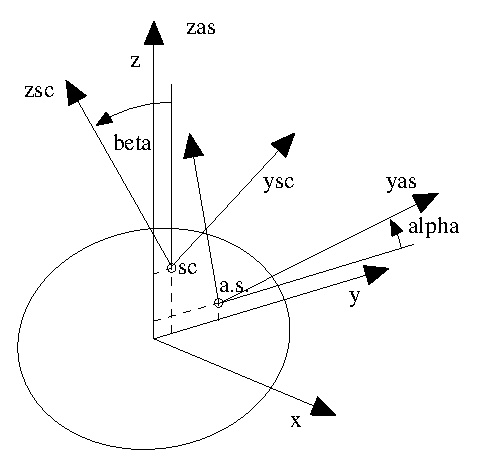
\includegraphics[width=.7\textwidth]{beamsect}
\caption{Beam section}
\label{fig:EL:BEAM:SECTION}
\end{figure}






\subsubsection{Generic Anisotropic Beam Section}
When a generic anisotropic beam section is considered,
the partitioning of axial and shear constitutive properties
of Figure~\ref{fig:EL:BEAM:GROUPS} is no longer possible.
The axial and shear straining can be completely and arbitrarily coupled,
resulting in a full constitutive matrix of the beam section,
\begin{align}
	\cubr{\cvvect{
		\T{f} \\
		\T{m}
	}}^\dagger
	&=
	\sqbr{\matr{cc}{
		\TT{K}_{\T{f}\T{\nu}} & \TT{K}_{\T{f}\T{\kappa}} \\
		\TT{K}_{\T{m}\T{\nu}} & \TT{K}_{\T{m}\T{\kappa}}
	}}^\dagger
	\cubr{\cvvect{
		\T{\nu} \\
		\T{\kappa}
	}}^\dagger ,
\end{align}
where $\T{f}$ and $\T{m}$ are the internal force and moment vectors,
while $\T{\nu}$ and $\T{\kappa}$ are the linear and angular strains.
Usually, $\TT{K}_{\T{m}\T{\nu}}\equiv\TT{K}_{\T{f}\T{\kappa}}^T$,
while $\TT{K}_{\T{f}\T{\nu}}$ and $\TT{K}_{\T{m}\T{\kappa}}$ are symmetric.


The reference point or the reference orientation of the constitutive
matrix can be changed by a sequence of transformations consisting
in a rotation and an offset.

The internal force and moment, after a rotation defined by the rotation
matrix $\TT{R}$, become
\begin{align}
	\cubr{\cvvect{
		\T{f} \\
		\T{m}
	}}^*
	&= \sqbr{\matr{cc}{
		\TT{R} & \TT{0} \\
		\TT{0} & \TT{R}
	}}
	\cubr{\cvvect{
		\T{f} \\
		\T{m}
	}}^\dagger
	.
\end{align}
Similarly, the strains become
\begin{align}
	\cubr{\cvvect{
		\T{\nu} \\
		\T{\kappa}
	}}^*
	&= \sqbr{\matr{cc}{
		\TT{R} & \TT{0} \\
		\TT{0} & \TT{R}
	}}^{-T}
	\cubr{\cvvect{
		\T{\nu} \\
		\T{\kappa}
	}}^\dagger
	\nonumber \\
	&= \sqbr{\matr{cc}{
		\TT{R} & \TT{0} \\
		\TT{0} & \TT{R}
	}}
	\cubr{\cvvect{
		\T{\nu} \\
		\T{\kappa}
	}}^\dagger
	.
\end{align}
As a consequence, the re-oriented constitutive relationship is
\begin{align}
	\cubr{\cvvect{
		\T{f} \\
		\T{m}
	}}^*
	&=
	\sqbr{\matr{cc}{
		\TT{R} & \TT{0} \\
		\TT{0} & \TT{R}
	}}
	\sqbr{\matr{cc}{
		\TT{K}_{\T{f}\T{\nu}} & \TT{K}_{\T{f}\T{\kappa}} \\
		\TT{K}_{\T{m}\T{\nu}} & \TT{K}_{\T{m}\T{\kappa}}
	}}^\dagger
	\sqbr{\matr{cc}{
		\TT{R} & \TT{0} \\
		\TT{0} & \TT{R}
	}}^T
	\cubr{\cvvect{
		\T{\nu} \\
		\T{\kappa}
	}}^*
	\nonumber \\
	&=
	\sqbr{\matr{cc}{
		\TT{R} \TT{K}_{\T{f}\T{\nu}}^\dagger \TT{R}^T
			& \TT{R} \TT{K}_{\T{f}\T{\kappa}}^\dagger \TT{R}^T \\
		\TT{R} \TT{K}_{\T{m}\T{\nu}}^\dagger \TT{R}^T
			& \TT{R} \TT{K}_{\T{m}\T{\kappa}}^\dagger \TT{R}^T
	}}
	\cubr{\cvvect{
		\T{\nu} \\
		\T{\kappa}
	}}^*
	\nonumber \\
	&=
	\sqbr{\matr{cc}{
		\TT{K}_{\T{f}\T{\nu}} & \TT{K}_{\T{f}\T{\kappa}} \\
		\TT{K}_{\T{m}\T{\nu}} & \TT{K}_{\T{m}\T{\kappa}}
	}}^*
	\cubr{\cvvect{
		\T{\nu} \\
		\T{\kappa}
	}}^*
	.
\end{align}

The internal moment, after considering an offset $\T{o}=\sqbr{0, y, z}^T$
of the reference point of the constitutive properties, becomes
$\T{m}=\T{m}^* + \T{o}\times\T{f}^*$.
The internal force and moment then becomes
\begin{align}
	\cubr{\cvvect{
		\T{f} \\
		\T{m}
	}}
	&= \sqbr{\matr{cc}{
		\TT{I} & \TT{0} \\
		\T{o}\times{} & \TT{I}
	}}
	\cubr{\cvvect{
		\T{f} \\
		\T{m}
	}}^*
	\label{eq:EL:BEAM:ANISOTROPIC-T}
	.
\end{align}
Similarly, the linear and angular strain vectors become
\begin{align}
	\cubr{\cvvect{
		\T{\nu} \\
		\T{\kappa}
	}}
	&= \sqbr{\matr{cc}{
		\TT{I} & \TT{0} \\
		\T{o}\times{} & \TT{I}
	}}^{-T}
	\cubr{\cvvect{
		\T{\nu} \\
		\T{\kappa}
	}}^*
	.
\end{align}
As a consequence, the offset constitutive relationship becomes
\begin{align}
	\cubr{\cvvect{
		\T{f} \\
		\T{m}
	}}
	&=
	\sqbr{\matr{cc}{
		\TT{I} & \TT{0} \\
		\T{o}\times{} & \TT{I}
	}}
	\sqbr{\matr{cc}{
		\TT{K}_{\T{f}\T{\nu}} & \TT{K}_{\T{f}\T{\kappa}} \\
		\TT{K}_{\T{m}\T{\nu}} & \TT{K}_{\T{m}\T{\kappa}}
	}}^*
	\sqbr{\matr{cc}{
		\TT{I} & \T{o}\times{}^T \\
		\TT{0} & \TT{I}
	}}
	\cubr{\cvvect{
		\T{\nu} \\
		\T{\kappa}
	}}
	\nonumber \\
	&=
	\sqbr{\matr{cc}{
		\TT{K}_{\T{f}\T{\nu}}^*
		& \TT{K}_{\T{f}\T{\nu}}^* \T{o}\times{}^T
			+ \TT{K}_{\T{f}\T{\kappa}}^* \\
		\T{o}\times\TT{K}_{\T{f}\T{\nu}}^*
			+ \TT{K}_{\T{m}\T{\nu}}^*
		& \T{o}\times\TT{K}_{\T{f}\T{\nu}}^* \T{o}\times{}^T
			+ \TT{K}_{\T{m}\T{\nu}}^* \T{o}\times{}^T
			+ \T{o}\times\TT{K}_{\T{f}\T{\kappa}}^*
			+ \TT{K}_{\T{m}\T{\kappa}}^*
	}}
	\cubr{\cvvect{
		\T{\nu} \\
		\T{\kappa}
	}}
	\nonumber \\
	&=
	\sqbr{\matr{cc}{
		\TT{K}_{\T{f}\T{\nu}} & \TT{K}_{\T{f}\T{\kappa}} \\
		\TT{K}_{\T{m}\T{\nu}} & \TT{K}_{\T{m}\T{\kappa}}
	}}
	\cubr{\cvvect{
		\T{\nu} \\
		\T{\kappa}
	}}^*
	.
\end{align}

It might be tempting to find what offset and rotation allows
to decouple the force and moment constitutive properties.
This can be sought by defining a generic transformation
\begin{align}
	\cubr{\cvvect{
		\T{f} \\
		\T{m}
	}}
	&= \sqbr{\matr{cc}{
		\TT{I} & \TT{0} \\
		\TT{T} & \TT{I}
	}}
	\cubr{\cvvect{
		\T{f} \\
		\T{m}
	}}^\dagger
	,
\end{align}
such that
\begin{align}
	\cubr{\cvvect{
		\T{f} \\
		\T{m}
	}}
	&=
	\sqbr{\matr{cc}{
		\TT{I} & \TT{0} \\
		\TT{T} & \TT{I}
	}}
	\sqbr{\matr{cc}{
		\TT{K}_{\T{f}\T{\nu}} & \TT{K}_{\T{f}\T{\kappa}} \\
		\TT{K}_{\T{m}\T{\nu}} & \TT{K}_{\T{m}\T{\kappa}}
	}}^\dagger
	\sqbr{\matr{cc}{
		\TT{I} & \TT{T}^T \\
		\TT{0} & \TT{I}
	}}
	\cubr{\cvvect{
		\T{\nu} \\
		\T{\kappa}
	}}
	\nonumber \\
	&=
	\sqbr{\matr{cc}{
		\TT{K}_{\T{f}\T{\nu}}^\dagger
		& \TT{K}_{\T{f}\T{\nu}}^\dagger \TT{T}^T
			+ \TT{K}_{\T{f}\T{\kappa}}^\dagger \\
		\TT{T}\TT{K}_{\T{f}\T{\nu}}^\dagger
			+ \TT{K}_{\T{m}\T{\nu}}^\dagger
		& \TT{T}\TT{K}_{\T{f}\T{\nu}}^\dagger \TT{T}^T
			+ \TT{K}_{\T{m}\T{\nu}}^\dagger \TT{T}^T
			+ \TT{T}\TT{K}_{\T{f}\T{\kappa}}^\dagger
			+ \TT{K}_{\T{m}\T{\kappa}}^\dagger
	}}
	\cubr{\cvvect{
		\T{\nu} \\
		\T{\kappa}
	}}
	.
\end{align}
The expected decoupling results from
\begin{align}
	\TT{T}
	&= 
	- \TT{K}_{\T{m}\T{\nu}}^\dagger
		\plbr{\TT{K}_{\T{f}\T{\nu}}^\dagger}^{-1}
	.
\end{align}
However, the resulting transformation $\TT{T}$ is not guaranteed
to have the skew-symmetric structure of $\T{o}\times{}$,
thus the decoupling may not be reducible to an offset.

The reverse transformation is relatively straightforward, after noticing
that, according to Eq.~(\ref{eq:EL:BEAM:ANISOTROPIC-T}), 
\begin{align}
	\cubr{\cvvect{
		\T{f} \\
		\T{m}
	}}^*
	&= \sqbr{\matr{cc}{
		\TT{I} & \TT{0} \\
		\T{o}\times{} & \TT{I}
	}}^{-1}
	\cubr{\cvvect{
		\T{f} \\
		\T{m}
	}}
	\nonumber \\
	&= \sqbr{\matr{cc}{
		\TT{I} & \TT{0} \\
		-\T{o}\times{} & \TT{I}
	}}
	\cubr{\cvvect{
		\T{f} \\
		\T{m}
	}}
	.
\end{align}
So, as expected, it is sufficient to revert the sign of the offset
to revert the transformation.
The signs of the constitutive relationship change accordingly.


\subsubsection{Locking Correction for Two-Node Beam}
The three-node finite volume element has been implemented first, 
and uses conventional polynomial parabolic interpolation 
of the nodal displacements and orientations;
the two-node finite volume element has been introduced later.
This latter element presents some shear-locking, which, for linear elastic
constitutive laws, may be overcome by correcting the section stiffness matrix
in a relatively straightforward form:
\begin{equation}\label{eq:2-NODE-BEAM-STIFFNESS}
	\hat{\T{K}} = \plbr{\T{F} + \frac{L^2}{12}\T{T} \T{F} \T{T}^T}^{-1} ,
\end{equation}
where $\T{F}=\T{K}^{-1}$ is the compliance matrix of the section, 
$L$ is the length of the beam, i.e.\ the distance between
the two reference points obtained by adding the optional offset 
to the nodes, and
\begin{displaymath}
	\T{T} \ = \ \sqbr{\matr{cc}{
		\T{0} & \T{e}_x \times{} \\
		\T{0} & \T{0}
	}}
\end{displaymath}
is the ``arm'' matrix that appears in the differential equilibrium equation
\begin{displaymath}
	\T{\vartheta}_{/x} - \T{T}^T\T{\vartheta} + \T{\phi} = 0
	,
\end{displaymath}
where $\T{\vartheta}=\sqbr{\T{f}^T \T{m}^T}^T$ are the internal forces
and moments, while $\T{\phi}$ are the external forces and moments
per unit span.

There are no provisions to automatically apply the correction 
when defining the constitutive law of the section.
The two-node beam has been re-implemented using a helicoidal interpolation
of the nodal positions and orientations, to improve its capability
to undergo large displacements and relative rotations.
It is activated by using the keyword \kw{hbeam2} instead of \kw{beam2}.
However, to reduce the shear-locking effect, the stiffness properties 
still need to be manually corrected according
to Equation~(\ref{eq:2-NODE-BEAM-STIFFNESS}).
The \kw{hbeam2} element is \emph{experimental}, and should be used
only for development purposes.


\subsection{Three-node beam element}
\label{sec:EL:BEAM:BEAM3}
The three-node beam element is described in detail in \cite{FV-AIAA}.
Each of the three points the beam element connects is referred
to a structural node but can have an arbitrary offset
to allow high generality in locating the structural reference line
of the beam.
Figure~\ref{fig:EL:BEAM:beam3} illustrates the geometry
of the three-node beam element.

\begin{figure}
\centering
\psfrag{1}{1}
\psfrag{2}{2}
\psfrag{3}{3}
\psfrag{n1}{node 1}
\psfrag{n2}{node 2}
\psfrag{n3}{node 3}
\psfrag{pI}{point I}
\psfrag{pII}{point II}
\psfrag{o1}{$\T{o}_1$}
\psfrag{o2}{$\T{o}_2$}
\psfrag{o3}{$\T{o}_3$}
\psfrag{RI}{$\TT{R}_I$}
\psfrag{RII}{$\TT{R}_{II}$}
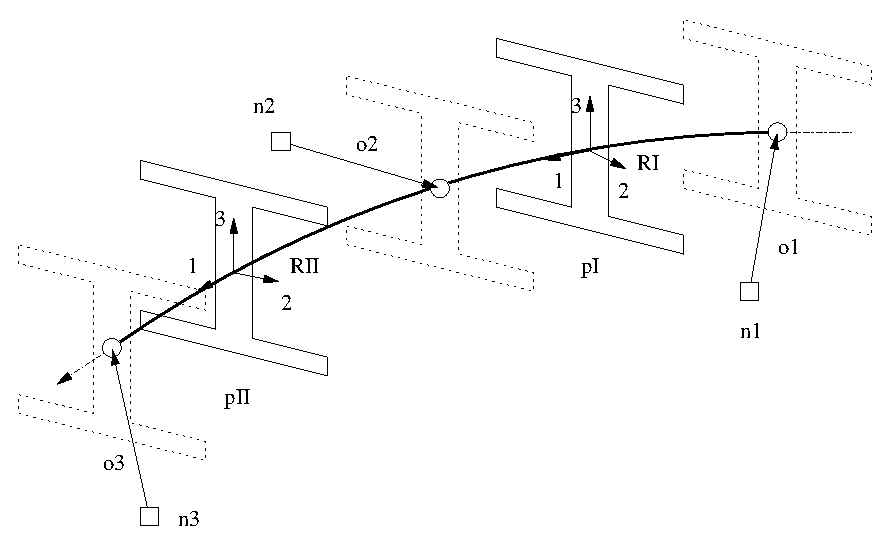
\includegraphics[width=.7\textwidth]{beam3}
\caption{Geometry of the three-node beam element.}
\label{fig:EL:BEAM:beam3}
\end{figure}

The finite volume formulation presented in \cite{FV-AIAA} is used.
As a consequence, the internal forces and moments are evaluated 
at two points that are at about midpoint between nodes 1 and 2, 
and nodes 2 and 3 (at $ \xi=-1/\sqrt{3}\cong -0.57735 $
and $\xi=1/\sqrt{3} \cong 0.57735$ of a non-dimensional abscissa $\xi$
running from $\xi=-1$ at node 1 to $\xi=1$ at node 3).

So the constitutive properties must be supplied in these points, as well as
the orientation matrices $\TT{R}_I$ and $\TT{R}_{II}$,
that express the orientation of the reference system
the constitutive properties are expressed in with respect to the global frame
(the axial force is conventionally defined in direction 1).
Any of the supported 6D constitutive laws can be supplied to define the
constitutive properties of each beam section.

The traditional input format is
%\begin{verbatim}
\begin{Verbatim}[commandchars=\\\{\}]
    \bnt{elem_type} ::= \kw{beam3}

    \bnt{normal_arglist} ::=
        \bnt{node_1_label} , (\hty{Vec3}) \bnt{relative_offset_1} ,
        \bnt{node_2_label} , (\hty{Vec3}) \bnt{relative_offset_2} ,
        \bnt{node_3_label} , (\hty{Vec3}) \bnt{relative_offset_3} ,
        (\hty{OrientationMatrix}) \bnt{orientation_matrix_section_I} ,
        (\htybkw{ConstitutiveLaw}{6D}) \bnt{constitutive_law_section_I} ,
        \{ \kw{same} | (\hty{OrientationMatrix}) \bnt{orientation_matrix_section_II} \} ,
        \{ \kw{same} | (\htybkw{ConstitutiveLaw}{6D}) \bnt{constitutive_law_section_II} \}
        [ , \bnt{custom_output} ]
\end{Verbatim}
%\end{verbatim}

The \nt{relative\_offset\_}\bnt{i}, with \nt{i}=1,2,3, are the vectors
$\T{o}_i$, with $i$=1,2,3, of Figure~\ref{fig:EL:BEAM:beam3}.

The orientation matrices \nt{orientation\_matrix\_section\_}\bnt{j},
with \nt{j}=I,II, are the section orientation matrices
$\TT{R}_j$, with $j$=$I$,$II$, of Figure~\ref{fig:EL:BEAM:beam3}.
They represent the (absolute) orientation in which the respective
constitutive properties are expressed.

The first keyword \kw{same}, alternative to the 
\nt{orientation\_matrix\_section\_II}, means that the same orientation
defined for the first point will be used for the second point.

The second keyword \kw{same}, alternative to the
\nt{constitutive\_law\_section\_II}, means that the same constitutive law
defined for the first point will be used for the second point.

If any of the constitutive laws is either viscous or viscoelastic,
the viscoelastic variant of the beam element is used.
Otherwise, the elastic variant is used.

A more complete input format is
%\begin{verbatim}
\begin{Verbatim}[commandchars=\\\{\}]
    \bnt{elem_type} ::= \kw{beam3}

    \bnt{normal_arglist} ::=
        \bnt{node_1_label} ,
            [ \kw{position} , ] (\hty{Vec3}) \bnt{relative_offset_1} ,
            [ \kw{orientation} , (\hty{OrientationMatrix}) \bnt{relative_orientation_1} , ]
        \bnt{node_2_label} ,
            [ \kw{position} , ] (\hty{Vec3}) \bnt{relative_offset_2} ,
            [ \kw{orientation} , (\hty{OrientationMatrix}) \bnt{relative_orientation_2} , ]
        \bnt{node_3_label} ,
            [ \kw{position} , ] (\hty{Vec3}) \bnt{relative_offset_3} ,
            [ \kw{orientation} , (\hty{OrientationMatrix}) \bnt{relative_orientation_3} , ]
        \{ (\hty{OrientationMatrix}) \bnt{orientation_matrix_section_I}
            | \kw{from nodes} \} ,
        (\htybkw{ConstitutiveLaw}{6D}) \bnt{constitutive_law_section_I} ,
        \{ \kw{same}
            | (\hty{OrientationMatrix}) \bnt{orientation_matrix_section_II}
            | \kw{from nodes} \} ,
        \{ \kw{same}
            | (\htybkw{ConstitutiveLaw}{6D}) \bnt{constitutive_law_section_II} \}
        [ , \bnt{custom_output} ]
\end{Verbatim}
%\end{verbatim}
This format is a superset of the traditional one, which is extended
by adding the possibility to set, for each node, the relative orientation
\nt{relative\_orientation\_}\bnt{i}, with \nt{i}=1,2,3,
with respect to the node itself.
Such orientation can be subsequently used to interpolate the orientation matrices
at the evaluation points, by providing the keyword \kw{from nodes}
instead of the orientation matrix.
If the keyword \kw{same} is used for the second evaluation point,
the same method is used to compute the orientation matrix.

The \nt{custom\_output} optional data consists in
%\begin{verbatim}
\begin{Verbatim}[commandchars=\\\{\}]
    \bnt{custom_output} ::= \kw{custom output} , \bnt{custom_output_flag} [ , ... ]
\end{Verbatim}
%\end{verbatim}
The values of \nt{custom\_output\_flag}
are defined in Section~\ref{sec:CONTROLDATA:DEFAULTBEAMOUTPUT}.

Flags add up to form the custom output request.
Flags may not be repeated.
Strain rates are only available from viscoelastic beams.
By default, only forces are output, to preserve compatibility
with the original output format.
The custom output is only available in NetCDF format;
see Section~\ref{sec:NetCDF:Elem:Beam}.

As an example, a simple beam element, with diagonal section stiffness 
matrix is presented:
\begin{verbatim}
    set: integer beam_label = 1000;
    set: integer beam_node1 = 2001;
    set: integer beam_node2 = 2002;
    set: integer beam_node3 = 2003;
    set: real EA = 1e6;   # N
    set: real GAy = .6e6; # N
    set: real GAz = .6e6; # N
    set: real GJ = 1.e3;  # Nm^2
    set: real EJy = 2.e3; # Nm^2
    set: real EJz = 1.e4; # Nm^2
    beam3: beam_label,
        beam_node1, reference, node, null,
        beam_node2, reference, node, null,
        beam_node3, reference, node, null,
        eye,
        linear elastic generic, diag,
            EA, GAy, GAz, GJ, EJy, EJz,
        same,
        same;
\end{verbatim}

A not-so-simple beam section, where the center of axial strain 
and the shear center are not coincident, is illustrated below.
The node offset is used to align the reference line 
with the shear center, and the axial strain center offset 
is used in the constitutive matrix:
\begin{verbatim}
    set: integer beam_label = 1000;
    set: integer beam_node1 = 2001;
    set: integer beam_node2 = 2002;
    set: integer beam_node3 = 2003;
    set: real EA = 1e6;    # N
    set: real GAy = .6e6;  # N
    set: real GAz = .6e6;  # N
    set: real GJ = 1.e3;   # Nm^2
    set: real EJy = 2.e3;  # Nm^2
    set: real EJz = 1.e4;  # Nm^2
    set: real yas = 2.e-2; # m
    set: real zas = 1.e-2; # m
    set: real ysc = 4.e-2; # m
    set: real zsc = 2.e-2; # m
    set: real y = yas-ysc; # compute the axial strain center
    set: real z = zas-zsc; # wrt/ the shear center
    beam3: beam_label,
        beam_node1, reference, node, 0.,ysc,zsc,
        beam_node2, reference, node, 0.,ysc,zsc,
        beam_node3, reference, node, 0.,ysc,zsc,
        eye,
        linear elastic generic, sym,
            EA, 0.,  0.,  0., z*EA,       -y*EA,
                GAy, 0.,  0., 0.,          0.,
                     GAz, 0., 0.,          0.,
                          GJ, 0.,          0.,
                              EJy+z^2*EA, -z*y*EA,
                                           EJz+y^2*EA,
        same,
        same;
\end{verbatim}


A piezoelectric actuator beam element is available; an arbitrary
linear piezoelectric actuation matrix is required, together with the labels
of the abstract nodes that represent the input signal tensions, as follows:
%\begin{verbatim}
\begin{Verbatim}[commandchars=\\\{\}]
    \bnt{normal_arglist} ::=
        \bnt{node_1_label} , (\hty{Vec3}) \bnt{relative_offset_1} ,
        \bnt{node_2_label} , (\hty{Vec3}) \bnt{relative_offset_2} ,
        \bnt{node_3_label} , (\hty{Vec3}) \bnt{relative_offset_3} ,
        (\hty{OrientationMatrix}) \bnt{orientation_matrix_section_I} ,
        (\htybkw{ConstitutiveLaw}{6D}) \bnt{constitutive_law_section_I} ,
        \{ \kw{same} | (\hty{OrientationMatrix}) \bnt{orientation_matrix_section_II} \} ,
        \{ \kw{same} | (\htybkw{ConstitutiveLaw}{6D}) \bnt{constitutive_law_section_II} \} ,
        \kw{piezoelectric actuator} , 
            \bnt{electrodes_number} ,
            \bnt{abstract_node_label_list} ,
            (\hty{Mat6xN}) \bnt{piezoelectric_matrix_I} ,
            \{ \kw{same} | (\hty{Mat6xN}) \bnt{piezoelectric_matrix_II} \}
        [ , \bnt{custom_output} ]
\end{Verbatim}
%\end{verbatim}
where the \nt{abstract\_node\_label\_list} is the list of the labels of the
abstract nodes that represent the electrodes.

A fully coupled piezoelectric beam element is available as well; an arbitrary
linear piezoelectric actuation matrix is required, together with the labels
of the abstract nodes that represent the input signal tensions, as follows:
%\begin{verbatim}
\begin{Verbatim}[commandchars=\\\{\}]
    \bnt{normal_arglist} ::=
        \bnt{node_1_label} , (\hty{Vec3}) \bnt{relative_offset_1} ,
        \bnt{node_2_label} , (\hty{Vec3}) \bnt{relative_offset_2} ,
        \bnt{node_3_label} , (\hty{Vec3}) \bnt{relative_offset_3} ,
        (\hty{OrientationMatrix}) \bnt{orientation_matrix_section_I} ,
        (\htybkw{ConstitutiveLaw}{6D}) \bnt{constitutive_law_section_I} ,
        \{ \kw{same} | (\hty{OrientationMatrix}) \bnt{orientation_matrix_section_II} \} ,
        \{ \kw{same} | (\htybkw{ConstitutiveLaw}{6D}) \bnt{constitutive_law_section_II} \} ,
        \kw{piezoelectric beam} , 
            \bnt{electrodes_number} ,
            \bnt{abstract_node_label_list} ,
            (\hty{Mat6xN}) \bnt{piezoelectric_matrix_I} ,
            (\hty{MatNx6}) \bnt{piezoelectric_charges_def_I} ,
            (\hty{MatNxN}) \bnt{piezoelectric_charges_potential_I} ,
            \{ 
                \kw{same}
               |
                (\hty{Mat6xN}) \bnt{piezoelectric_matrix_II} 
                (\hty{MatNx6}) \bnt{piezoelectric_charges_def_II} ,
                (\hty{MatNxN}) \bnt{piezoelectric_charges_potential_II}
            \}
        [ , \bnt{custom_output} ]
\end{Verbatim}
%\end{verbatim}
where the \nt{abstract\_node\_label\_list} is the list of the labels of the
abstract nodes that represent the electrodes, \nt{piezoelectric\_charges\_def} give
to compute the charge per unit of length as a function of the beam generalized
deformation measures, and \nt{piezoelectric\_charges\_potential} the charge per unit of length 
as a function of the electrodes potential.


\paragraph{Private Data}
\label{sec:EL:BEAM:PRIVATE}
The following data are available:
\begin{enumerate}
\item \kw{"ex"} axial strain
\item \kw{"ey"} shear strain (local axis 2)
\item \kw{"ez"} shear strain (local axis 3)
\item \kw{"kx"} curvature about local axis 1 (torsional)
\item \kw{"ky"} curvature about local axis 2 (bending)
\item \kw{"kz"} curvature about local axis 3 (bending)
\item \kw{"Fx"} axial force
\item \kw{"Fy"} shear force (direction 2)
\item \kw{"Fz"} shear force (direction 3)
\item \kw{"Mx"} moment about local axis 1 (torsional)
\item \kw{"My"} moment about local axis 2 (bending)
\item \kw{"Mz"} moment about local axis 3 (bending)
\item \kw{"Xx"} absolute position component 1
\item \kw{"Xy"} absolute position component 2
\item \kw{"Xz"} absolute position component 3
\item \kw{"Phix"} absolute orientation vector component 1
\item \kw{"Phiy"} absolute orientation vector component 2
\item \kw{"Phiz"} absolute orientation vector component 3
\item \kw{"Omegax"} absolute angular velocity component 1
\item \kw{"Omegay"} absolute angular velocity component 2
\item \kw{"Omegaz"} absolute angular velocity component 3
\item \kw{"ePx"} axial strain rate
\item \kw{"ePy"} shear strain rate (local axis 2)
\item \kw{"ePz"} shear strain rate (local axis 3)
\item \kw{"kPx"} curvature rate about local axis 1 (torsional)
\item \kw{"kPy"} curvature rate about local axis 2 (bending)
\item \kw{"kPz"} curvature rate about local axis 3 (bending)
\end{enumerate}
Each string is prefixed by \kw{"pI."} or \kw{"pII."}
to specify data related to either the first or the second point:
\begin{verbatim}
    "pI.Fx"     # axial force at point I
    "pII.kz"    # bending curvature about local axis 3 at point II
\end{verbatim}
Private data related to point I are numbered from 1 to 27;
private data related to point II are numbered from 28 to 54.



\subsubsection{Inertia Properties}
So-called ``consistent inertia'' is not implemented for beam elements; one needs to use \kw{body} (rigid-body) elements 
(Section~\ref{sec:EL:BODY}) instead.
Their suggested usage is detailed here.

In principle, from the inertial point of view, the beam should be split in ``chunks'' as discussed earlier.
Distributed inertia loads are associated with the motion of each chunk.
For moderate straining, one can safely assume that the chunks remain rigid with respect to inertia loads computation.

For the sake of simplicity, it is assumed that the beam is straight, with uniform inertia properties,
where the $x$ axis is the beam axis, and $y$ and $z$ are principal inertia axes of the section.
Moreover, it is assumed that the nodes are equally spaced (i.e.\ the mid-node is at midspan).

Consider the mass per unit span $m$, the inertia moment per unit span about the beam's axis, $i_{xx}$,
and those about the two remaining axes, $i_{yy}$, $i_{zz}$, with $i_{xx} = i_{yy} + i_{zz}$.
The length of the beam element is $\ell$.

According to the theory, the beam is cut at two stations, set at $\pm \ell/(2 \sqrt{3})$ from the mid-node.
As a consequence, the length of the middle chunk is $\ell_{\text{mid}} = \ell/\sqrt{3}$, whereas that of the end chunks is
$\ell_{\text{end}} = \ell (1 - 1/\sqrt{3})/2$.

The corresponding bodies are
\begin{verbatim}
# body associated with first end node
body: 1,
    1, # label of first end node
    m*ell_end, # mass associated with first end node
    reference, node, ell_end/2, 0., 0., # the center of mass of this chunk
                                        # is offset along the beam axis
    diag,
        i_xx*ell_end,
        i_yy*ell_end + m*ell_end^3/12, # i_yy may often be neglected
        i_zz*ell_end + m*ell_end^3/12; # i_zz may often be neglected

# body associated with mid-node
body: 2,
    2, # label of mid-node
    m*ell_mid, # mass associated with mid-node
    reference, node, null, # the center of mass of this chunk is at the node
    diag,
        i_xx*ell_mid,
        i_yy*ell_mid + m*ell_mid^3/12,
        i_zz*ell_mid + m*ell_mid^3/12;

# body associated with last end node
body: 3,
    3, # label of last end node
    m*ell_end,
    reference, node, -ell_end/2, 0., 0.,
    diag,
        i_xx*ell_end,
        i_yy*ell_end + m*ell_end^3/12,
        i_zz*ell_end + m*ell_end^3/12;
\end{verbatim}
Often, $i_{yy}$ and $i_{zz}$ can be neglected, significantly when the beam element is slender enough
(i.e.\ when $\ell \sqrt{m A/i_{yy}} \approx \ell \sqrt{m A/i_{zz}} \ll 1$).

Moreover, the chunks do not necessarily need to be cut exactly at $\pm \ell / (2 \sqrt{3})$;
setting $\ell_{\text{mid}} = \ell/2$ and $\ell_{\text{end}} = \ell/4$ gives good results.

When assembling strings of beam elements, one would need to connect two \kw{body} elements to each end node,
each of them accounting from the inertial contribution of the two adjacent beam elements.
Alternatively, a single \kw{body} can be used, which accounts for the contribution of the two elements.
If the two adjacent beam elements are identical (i.e.\ same inertia properties, same length $\ell$),
an end body would look like
\begin{verbatim}
body: 3,
    3, # label of last end node
    m*(2*ell_end),
    reference, node, null,
    diag,
        i_xx*(2*ell_end),
        i_yy*(2*ell_end) + m*(2*ell_end)^3/12,
        i_zz*(2*ell_end) + m*(2*ell_end)^3/12;
\end{verbatim}
If the two adjacent beam elements differ, one can use the \kw{condense} option
to collect the inertia contributions from each beam element and let the solver
do the merge.
See Section~\ref{sec:EL:BODY} for more details.

If the beam element is significantly curved, one needs to evaluate the correct position of the center of mass,
and correct the inertia tensor accordingly.

If axes $y$, $z$ are not principal inertia axes, one needs to take into account the cross-coupling terms in the inertia tensor.





\subsection{Two-node beam element}
\label{sec:EL:BEAM:BEAM2}
Similar considerations apply to the two-node beam.
Its geometry is illustrated in Figure~\ref{fig:EL:BEAM:beam2}.

\begin{figure}
\centering
\psfrag{1}{1}
\psfrag{2}{2}
\psfrag{3}{3}
\psfrag{n1}{node 1}
\psfrag{n2}{node 2}
\psfrag{pI}{point I}
\psfrag{o1}{$\T{o}_1$}
\psfrag{o2}{$\T{o}_2$}
\psfrag{RI}{$\TT{R}_I$}
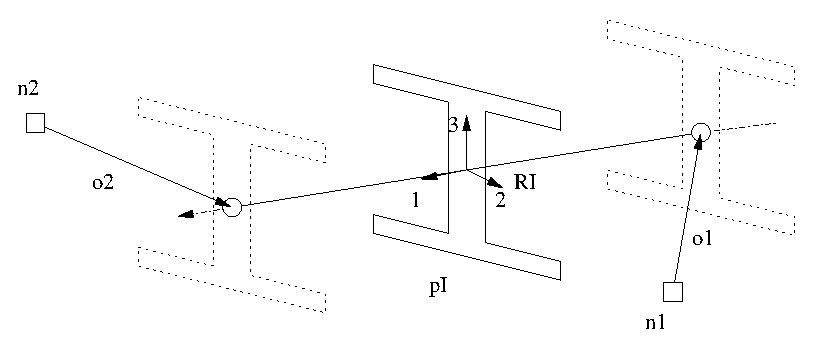
\includegraphics[width=.7\textwidth]{beam2}
\caption{Geometry of the two-node beam element.}
\label{fig:EL:BEAM:beam2}
\end{figure}

The syntax is
%\begin{verbatim}
\begin{Verbatim}[commandchars=\\\{\}]
    \bnt{elem_type} ::= \kw{beam2}

    \bnt{normal_arglist} ::=
        \bnt{node_1_label} , (\hty{Vec3}) \bnt{relative_offset_1} ,
        \bnt{node_2_label} , (\hty{Vec3}) \bnt{relative_offset_2} ,
        (\hty{OrientationMatrix}) \bnt{orientation_matrix_section_I} ,
        (\htybkw{ConstitutiveLaw}{6D}) \bnt{constitutive_law_section_I}
        [ , \kw{piezoelectric actuator} , 
            \bnt{electrodes_number} ,
            \bnt{abstract_node_label_list} ,
            (\hty{Mat6xN}) \bnt{piezoelectric_matrix_I} ]
        [ , \bnt{custom_output} ]
\end{Verbatim}
%\end{verbatim}

A more complete form is
%\begin{verbatim}
\begin{Verbatim}[commandchars=\\\{\}]
    \bnt{elem_type} ::= \kw{beam2}

    \bnt{normal_arglist} ::=
        \bnt{node_1_label} ,
            [ \kw{position} , ] (\hty{Vec3}) \bnt{relative_offset_1} ,
            [ \kw{orientation} , (\hty{OrientationMatrix}) \bnt{relative_orientation_1} , ]
        \bnt{node_2_label} ,
            [ \kw{position} , ] (\hty{Vec3}) \bnt{relative_offset_2} ,
            [ \kw{orientation} , (\hty{OrientationMatrix}) \bnt{relative_orientation_2} , ]
        \{ (\hty{OrientationMatrix}) \bnt{orientation_matrix_section_I}
            | \kw{from nodes} \} ,
        (\htybkw{ConstitutiveLaw}{6D}) \bnt{constitutive_law_section_I}
        [ , \kw{piezoelectric actuator} , 
            \bnt{electrodes_number} ,
            \bnt{abstract_node_label_list} ,
            (\hty{Mat6xN}) \bnt{piezoelectric_matrix_I} ]
        [ , \bnt{custom_output} ]
\end{Verbatim}
%\end{verbatim}

\paragraph{Private Data.}
The same private data indicated for the \kw{beam3} element is available
(see Section~\ref{sec:EL:BEAM:PRIVATE}).
No prefix must be specified (\kw{"pI."} is implicit).


\paragraph{Example.} \
As an example, a simple beam element, with diagonal section stiffness 
matrix is presented:
\begin{verbatim}
    set: integer beam_label = 1000;
    set: integer beam_node1 = 2001;
    set: integer beam_node2 = 2002;
    set: real L = .4;     # m
    set: real EA = 1e6;   # N
    set: real GAy = .6e6; # N
    set: real GAz = .6e6; # N
    set: real GJ = 1.e3;  # Nm^2
    set: real EJy = 2.e3; # Nm^2
    set: real EJz = 1.e4; # Nm^2
    beam2: beam_label,
        beam_node1, reference, node, null,
        beam_node2, reference, node, null,
        eye,
        linear elastic generic, diag,
            EA, 1./(1./GAy+L^2/12./EJz), 1./(1./GAz+L^2/12./EJy),
            GJ, EJy, EJz;
\end{verbatim}
Note that the shear terms have been na\"{\i}vely inverted to eliminate
shear locking, according to Equation~(\ref{eq:2-NODE-BEAM-STIFFNESS}).


\subsubsection{Inertia Properties}
According to the theory, the beam is cut in half.
As a consequence, the length of each chunk is $\ell_{\text{end}} = \ell/2$.

With reference to the symbols defined for the three-node beam element, the corresponding bodies are
\begin{verbatim}
# body associated with first end node
body: 1,
    1, # label of first end node
    m*ell_end, # mass associated with first end node
    reference, node, ell_end/2, 0., 0., # the center of mass of this chunk
                                        # is offset along the beam axis
    diag,
        i_xx*ell_end,
        i_yy*ell_end + m*ell_end^3/12, # i_yy may often be neglected
        i_zz*ell_end + m*ell_end^3/12; # i_zz may often be neglected

# body associated with last end node
body: 2,
    2, # label of last end node
    m*ell_end,
    reference, node, -ell_end/2, 0., 0.,
    diag,
        i_xx*ell_end,
        i_yy*ell_end + m*ell_end^3/12,
        i_zz*ell_end + m*ell_end^3/12;
\end{verbatim}
Similar considerations to those made for the three-node beam element apply also in this case.



\subsection{Output}
The output related to beam elements is contained in a file with extension 
\texttt{.act}; for each time step, the output is written
for those element it was requested.
The internal forces and moments are computed from the interpolated strains
along the beam by means of the constitutive law, at the evaluation points. 
The format is:
\begin{itemize}
    \item column 1: the label of the beam;
    \item columns 2--4: the three components of the force
	at the first evaluation point, oriented according
	to the reference frame of that beam section;
    \item columns 5--7: the three components of the moment
	at the first evaluation point, oriented according
	to the reference frame of that beam section.
\end{itemize}

The three-node beam element generates six additional columns:
\begin{itemize}
    \item columns 8--10: the three components of the force
	at the second evaluation point, oriented according
	to the reference frame of that beam section;
    \item columns 11--13: the three components of the moment
	at the second evaluation point, oriented according
	to the reference frame of that beam section.
\end{itemize}

More detailed output is allowed when using NetCDF;
see Section~\ref{sec:NetCDF:Elem:Beam} for details.



\subsection{Notes}
Two-node beam elements should be used with care.
